\documentclass{article}

\usepackage[utf8]{inputenc}
\usepackage[spanish]{babel}
\usepackage{graphicx}
\usepackage{amsmath}
\title{Modelos matemáticos discretos}
\author{Uriel Alejandro Nolasco Hernández}	
\begin{document}
	\maketitle
	\section{Ecuaciones en diferencias}

	\subsection{Primer Orden}
	Tenemos \$1000 que vamos a invertir a un interés del 1\% mensual.
El valor de la inversión cuando han tanscurrido $n$ meses es $$x_n=1000(1.01)^n$$

\begin{center}
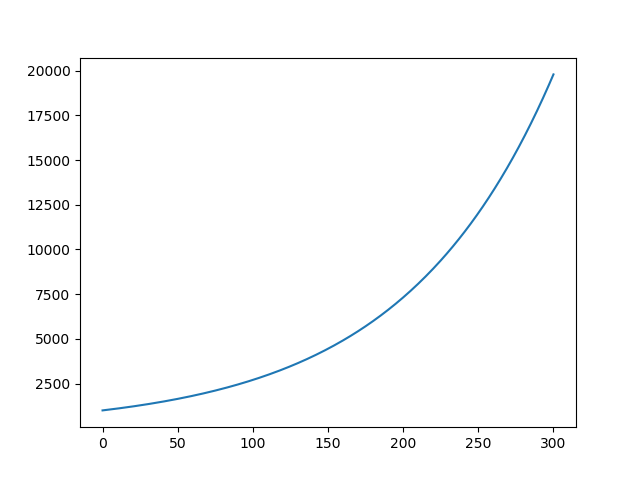
\includegraphics[width=8cm]{Figure_1}	
\end{center}
\end{document}

